\documentclass[12pt,a4paper]{article}
\usepackage[utf8]{inputenc}
\usepackage{times}
\usepackage{amsmath}
\usepackage{amssymb}
\usepackage{graphicx}
\usepackage{cite}
\usepackage{url}
\usepackage{hyperref}
\usepackage{geometry}
\usepackage{setspace}
\usepackage{indentfirst}
\usepackage{fancyhdr}
\usepackage[font={it,footnotesize}]{caption}
\usepackage{sectsty}
\usepackage{booktabs}
\usepackage{tikz}
\usetikzlibrary{shapes.geometric, arrows, positioning, fit, calc}

% Section title formatting
\sectionfont{\fontsize{12}{15}\selectfont\bfseries}
\subsectionfont{\fontsize{12}{15}\selectfont\bfseries}

% Page style
\pagestyle{fancy}
\fancyhf{}
\fancyfoot[C]{\thepage}
\renewcommand{\headrulewidth}{0pt}

% Margins and spacing
\geometry{left=2.54cm,right=2.54cm,top=2.54cm,bottom=2.54cm}
\renewcommand{\baselinestretch}{1.5}
\setlength{\parindent}{0.5cm}

% Title
\title{\fontsize{14}{17}\selectfont\textbf{Advances in Deep Learning for Remote Sensing Image Classification: A Comprehensive Review}}
\author{Liang Jingyu\\
        Northwestern Polytechnical University\\
        Xi'an, Shaanxi, China\\
        \texttt{3445078775@qq.com}}
\date{}

\begin{document}

\maketitle

\begin{abstract}
Deep neural networks have completely changed how we analyze images from satellites and aircraft. Today, carefully designed layered models achieve accuracies that were once unthinkable. They excel at difficult jobs like understanding entire scenes, finding precise object positions, or labeling every single pixel with meaning. Much of this success comes from better ways to handle features at different scales, from smart attention systems that highlight what truly matters, and from cleverly reusing parameters learned on other datasets.

Still, serious problems remain. Labeled data is painfully scarce. Training and running these models demands huge computing power, which makes deployment on satellites or drones very difficult. Models also struggle when lighting, weather, seasons, or sensor types change.

Researchers are responding in several promising directions. Many now pre-train networks on massive unlabeled collections without any human annotation. Others combine optical, radar, elevation, and hyperspectral data in more intelligent ways. At the same time, engineers keep pushing for smaller, faster networks that preserve most of the accuracy. These efforts together open real possibilities for practical, widespread use in a field that moves incredibly fast.
\end{abstract}

\textbf{Keywords:} Deep learning, Remote sensing, Image classification, Convolutional neural networks, Scene classification, Object detection

\section{Introduction}
\label{sec:introduction}

Over the past few years, remote sensing has changed dramatically. Networks of satellites, aircraft, and ground stations now deliver enormous volumes of high-resolution imagery every day. These pictures carry rich spectral, spatial, and temporal information. They support everything from land-use mapping and city planning to emergency response and climate monitoring. Yet the sheer amount and complexity of the data quickly overwhelmed older classification methods.

In the past, researchers relied heavily on hand-crafted features. They carefully designed descriptors based on spectral values, texture patterns, or geometric shapes. Those approaches worked reasonably well for simpler problems. However, they often failed when scenes became crowded or imaging conditions varied. Manual engineering also required deep expertise and took considerable time, so adapting to new sensors or tasks was slow and painful.

Deep learning changed the game. Instead of designing features by hand, networks now learn them directly from raw pixels. Convolutional neural networks proved especially powerful. They naturally capture spatial relationships and contextual information that earlier methods missed.

Remote sensing images, though, differ from ordinary photographs in important ways. They usually contain many spectral bands. Resolution varies widely across platforms. Scenes are often packed with objects of different sizes and complex layouts. And labeled examples remain expensive to produce. Because of these differences, the community has developed specialized architectures and training strategies that fit remote sensing needs much better.

This review surveys the most important advances made between 2020 and 2023. We first recall basic concepts in Section 2. Section 3 examines recent architectural improvements. Section 4 discusses three major application areas—scene classification, object detection, and semantic segmentation. Section 5 identifies remaining challenges and likely future directions. Section 6 concludes the paper.

\begin{table}[htbp]
\centering
\caption{Overview of Deep Learning Applications in Remote Sensing}
\label{tab:applications}
\begin{tabular}{@{}lll@{}}
\toprule
\textbf{Application}          & \textbf{Primary Task}         & \textbf{Key Challenge}      \\
\midrule
Scene Classification          & Image-level labeling          & Multi-scale features        \\
Object Detection              & Localization \& recognition   & Small object detection      \\
Semantic Segmentation         & Pixel-level classification   & Class imbalance             \\
\bottomrule
\end{tabular}
\end{table}

\section{Background}
\label{sec:background}

\subsection{Convolutional Neural Networks Fundamentals}

Convolutional neural networks were built specifically for grid-like data such as images. A typical network stacks convolutional layers, pooling operations, and fully connected layers, with non-linear activations sprinkled throughout.

Convolutional layers act as feature detectors. Each filter slides across the input and responds to local patterns—edges, corners, textures. Because the same filter is used everywhere, the number of parameters stays manageable. Pooling then reduces spatial size while keeping the most active responses. This makes the representation more robust to small shifts and cuts computation dramatically. Figure~\ref{fig:architecture} shows the usual pipeline in remote sensing work.

After several such stages, high-level features reach the final fully connected layers that produce class scores or bounding boxes. ReLU has become the default activation because it trains faster and suffers less from vanishing gradients than sigmoid or tanh.

\subsection{CNN Training and Optimization}

Training minimizes the difference between predictions and ground truth. Back-propagation computes gradients, and optimizers like SGD or Adam update weights. Several tricks have become standard to make training more stable and effective.

Data augmentation creates variations—rotations, flips, color jitter—so the network never sees exactly the same image twice. Dropout and weight decay prevent overfitting. Batch normalization stabilizes learning by normalizing activations inside each mini-batch. Transfer learning, perhaps the single most useful technique in remote sensing, starts from weights pre-trained on ImageNet and fine-tunes on the usually much smaller target dataset.

\subsection{Challenges Specific to Remote Sensing}

Remote sensing imagery poses difficulties that ordinary photos do not. First, images often have ten or more spectral bands, so input channels must be extended. Second, ground sampling distance varies greatly, so objects appear at very different scales. Third, scenes are semantically dense; a single patch may contain roads, buildings, trees, cars, and water bodies arranged in complicated ways. Fourth, accurate pixel-level or object-level labels are costly to obtain, so datasets are usually small compared to computer vision benchmarks. Finally, strong class imbalance is common—forests cover far more area than airports.

These peculiarities explain why generic ImageNet models rarely work well out-of-the-box and why the community has invested heavily in tailored solutions.

\section{Developments in CNN Architectures for Remote Sensing}
\label{sec:developments}

\subsection{Multi-scale Feature Extraction}

Objects in aerial and satellite images range from individual cars to entire cities. Fixed receptive fields of standard backbones therefore miss either fine details or global layout. Researchers have responded with several effective strategies.

Pyramid pooling modules apply pooling at multiple grid sizes and concatenate the results, giving the network both local and global cues in one shot. Dilated convolutions with different rates achieve similar effect without losing resolution. Feature pyramid networks build a proper hierarchy: high-level semantic features from deep layers are gradually merged with high-resolution shallow features through lateral connections. The resulting maps are semantically strong at every scale, which proves especially helpful for detecting tiny objects.

\subsection{Attention Mechanisms}

Attention has become almost ubiquitous. Spatial attention learns where to look, producing a soft mask that emphasizes discriminative regions and suppresses background clutter. Channel attention, exemplified by the squeeze-and-excitation block, re-weights entire feature maps according to their global importance. Combining both in sequence—convolutional block attention module—often yields the best gains.

In complex airport or harbor scenes, attention helps the model ignore large uniform areas (sea, runway) and focus on ships or planes that actually determine the scene category.

\subsection{Transfer Learning and Domain Adaptation}

Because labeled remote sensing data is limited, almost every published work starts from ImageNet-pre-trained backbones. Simple fine-tuning already brings huge improvements. Yet the domain gap between natural photos and overhead views remains large. Adversarial domain adaptation, correlation alignment, and self-training on pseudo-labels have all been used successfully to close that gap further.

\subsection{Lightweight Network Designs}

Satellites and drones have strict limits on power, memory, and computation. Standard ResNet-101 or EfficientNet models are simply too heavy. Depthwise separable convolutions cut computation roughly nine times with only minor accuracy loss. MobileNet, ShuffleNet, and GhostNet series therefore appear frequently in recent onboard processing papers. Neural architecture search has also discovered surprisingly efficient topologies that outperform hand-designed lightweight models under the same latency budget.

\section{Application Cases}
\label{sec:applications}

\begin{table}[h!]
\centering
\caption{Comparison of Major Deep Learning Tasks in Remote Sensing}
\label{tab:task_comparison}
\resizebox{\textwidth}{!}{%
\begin{tabular}{@{}llll@{}}
\toprule
\textbf{Task}                 & \textbf{Description}                                      & \textbf{Common Architectures}                          & \textbf{Key Challenges}                       \\
\midrule
Scene Classification          & Categorize an image based on its overall content         & CNNs with global average pooling, Multi-scale networks & Intra-class diversity, Inter-class similarity \\
Object Detection              & Locate and identify specific objects (e.g., vehicles)     & Faster R-CNN, YOLO, SSD, Rotated BBox methods          & Small object sizes, Varying orientations, Dense objects \\
Semantic Segmentation         & Assign a class label to every pixel in an image           & FCN, U-Net, DeepLab, Encoder-Decoder models            & Fine detail preservation, Class imbalance, Edge refinement \\
\bottomrule
\end{tabular}%
}
\end{table}

\subsection{Scene Classification}

Assigning one label to an entire overhead image sounds simple, but scenes are highly composite. A residential area may contain houses, roads, trees, cars, pools—yet must be distinguished from commercial or industrial areas with different spatial arrangements of similar elements.

Current best practice combines global context with local object cues. Some works extract object proposals first and then aggregate their features; others use multi-branch networks with different dilation rates. Attention almost always helps, especially when classes are visually similar (different types of airports, harbors, or storage tanks).

\subsection{Object Detection}

Finding and classifying cars, planes, ships, or buildings from above is hard because objects are usually small, arbitrarily oriented, and densely packed. Two-stage detectors like Faster R-CNN remain accurate but slow. Single-stage detectors—YOLOv5/8, SSD, RetinaNet, and their rotated variants—now dominate when speed matters. Most recent papers add feature pyramid modules, rotatable anchors or regression branches, and sometimes even keypoint-based representations to handle arbitrary orientations gracefully.

\subsection{Semantic Segmentation}

Pixel-level mapping is essential for producing clean land-cover or change-detection maps. Fully convolutional networks replaced the final classification layers with 1×1 convolutions so the network can process images of any size. U-Net added skip connections that bring back fine details lost during down-sampling (Figure~\ref{fig:unet_architecture}). DeepLab introduced atrous convolutions and pyramid pooling to enlarge receptive fields without losing resolution. Post-processing with fully connected CRFs or morphological operations further sharpens boundaries.

\begin{figure}[h!]
\centering
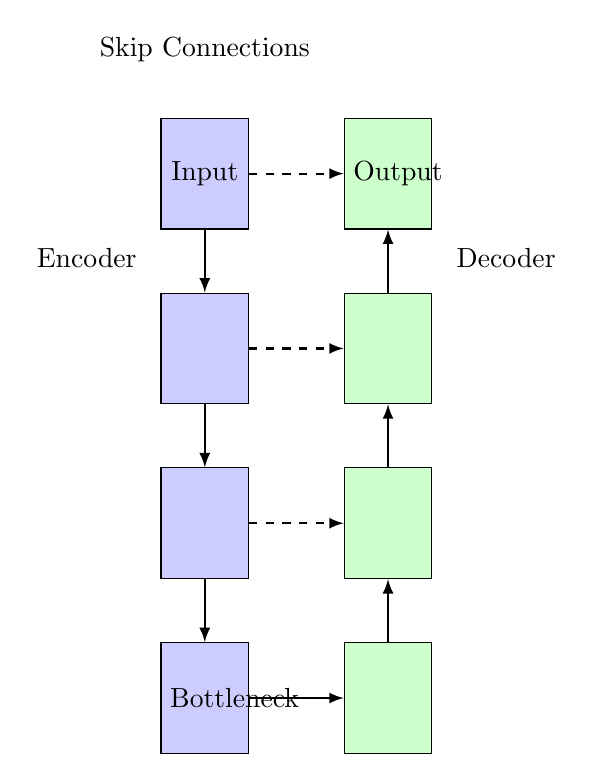
\begin{tikzpicture}[
    node distance=0.8cm and 1.2cm,
    block/.style={rectangle, draw, fill=blue!20, text width=2.5em, text centered, minimum height=4em},
    dblock/.style={rectangle, draw, fill=green!20, text width=2.5em, text centered, minimum height=4em},
    arrow/.style={-latex, thick}
]
    \node[block] (e1) {Input};
    \node[block, below=of e1] (e2) {};
    \node[block, below=of e2] (e3) {};
    \node[block, below=of e3] (e4) {Bottleneck};

    \node[dblock, right=of e4] (d4) {};
    \node[dblock, above=of d4] (d3) {};
    \node[dblock, above=of d3] (d2) {};
    \node[dblock, above=of d2] (d1) {Output};

    \draw[arrow] (e1) -- (e2);
    \draw[arrow] (e2) -- (e3);
    \draw[arrow] (e3) -- (e4);
    \draw[arrow] (e4) -- (d4);
    \draw[arrow] (d4) -- (d3);
    \draw[arrow] (d3) -- (d2);
    \draw[arrow] (d2) -- (d1);

    \draw[arrow, dashed] (e3.east) to [out=0,in=180] (d3.west);
    \draw[arrow, dashed] (e2.east) to [out=0,in=180] (d2.west);
    \draw[arrow, dashed] (e1.east) to [out=0,in=180] (d1.west);
    
    \node[above=0.2cm of e2, xshift=-1.5cm, align=center] {Encoder};
    \node[above=0.2cm of d2, xshift=1.5cm, align=center] {Decoder};
    \node[above=0.1cm of d2, midway, yshift=1.2cm] {Skip Connections};
\end{tikzpicture}
\caption{A simplified diagram of the U-Net architecture, showing the symmetric encoder-decoder pathways and the skip connections that merge high-resolution features from the encoder with upsampled features in the decoder.}
\label{fig:unet_architecture}
\end{figure}

\section{Challenges and Future Directions}
\label{sec:challenges}

\subsection{Limited Training Data}

Even today, high-quality labels remain the biggest bottleneck. Self-supervised pretraining on huge unlabeled archives has therefore attracted massive interest. Contrastive methods (MoCo, SwAV, DINO) and masked image modeling (MAE, SimMIM) now produce features that rival or surpass ImageNet supervision when fine-tuned on downstream remote sensing tasks.

Weakly supervised and semi-supervised approaches also help. Image-level tags, scribbles, or point annotations cost far less than pixel-level masks yet can train surprisingly strong segmentation models when combined cleverly.

\subsection{Computational Efficiency}

Onboard real-time processing demands models under 100 MB with inference times of tens of milliseconds. Pruning, quantization, distillation, and efficient attention variants all contribute. Hardware-aware neural architecture search is beginning to produce networks specifically optimized for satellite or UAV chips.

\subsection{Multi-modal Data Fusion}

Optical images fail at night or in clouds. SAR and LiDAR work in any weather but lack rich color information. Learning how to combine them effectively is still an open problem. Early fusion is simple but brittle. Late fusion is robust but misses cross-modal interactions. Middle fusion with cross-attention or shared transformers currently shows the most promise.

\subsection{Interpretability and Explainability}

In operational use, stakeholders need to understand why a model classified a certain area as “damaged” after a disaster. Grad-CAM and attention rollout visualizations are routinely included in recent papers. Concept-based methods that link network activations to human-readable concepts (vegetation index, roof material, etc.) are emerging but not yet mature.

\begin{figure}[htbp]
\centering
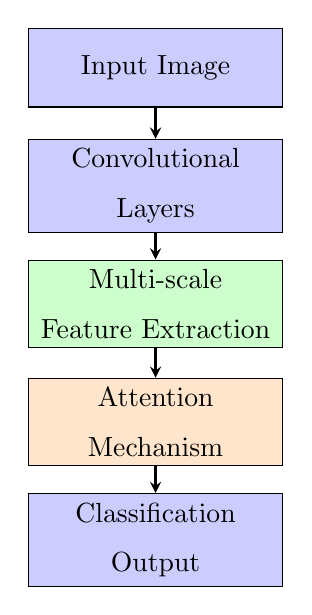
\begin{tikzpicture}[
    node distance=1.5cm,
    box/.style={rectangle, draw, fill=blue!20, text width=3cm, align=center, minimum height=1cm},
    arrow/.style={->, >=stealth, thick}
]
    \node[box] (input) {Input Image};
    \node[box, below of=input] (conv) {Convolutional Layers};
    \node[box, below of=conv, fill=green!20] (multiscale) {Multi-scale Feature Extraction};
    \node[box, below of=multiscale, fill=orange!20] (attention) {Attention Mechanism};
    \node[box, below of=attention] (output) {Classification Output};
    
    \draw[arrow] (input) -- (conv);
    \draw[arrow] (conv) -- (multiscale);
    \draw[arrow] (multiscale) -- (attention);
    \draw[arrow] (attention) -- (output);
\end{tikzpicture}
\caption{General architecture of deep learning models for remote sensing image classification}
\label{fig:architecture}
\end{figure}

\section{Conclusion}
\label{sec:conclusion}

Between 2020 and 2023 the field witnessed remarkable progress. Multi-scale feature fusion, attention mechanisms, better transfer strategies, and lightweight designs have together pushed accuracy to levels that enable real operational deployment. Yet labeled data scarcity, computational constraints, multi-modal integration, and interpretability issues continue to limit broader adoption.

Looking ahead, self-supervised and foundation models trained on billions of unlabeled satellite images will likely reduce annotation needs dramatically. Efficient architectures tailored for edge devices will appear more often. Smarter ways to fuse optical, SAR, hyperspectral, and temporal data will unlock new applications. And interpretability techniques will mature so that decisions become trustworthy in critical scenarios.

Remote sensing is producing more data every year. Deep learning, properly adapted to its unique challenges, is the tool best positioned to turn that flood of pixels into actionable knowledge.

\begin{table}[htbp]
\centering
\caption{Comparison of Deep Learning Approaches for Remote Sensing}
\label{tab:comparison}
\begin{tabular}{@{}llll@{}}
\toprule
\textbf{Method}       & \textbf{Strength}         & \textbf{Limitation}       & \textbf{Best Use Case}   \\
\midrule
CNN-based             & High accuracy             & Large data needed         & Scene classification    \\
Attention-based       & Feature selection         & Computational cost        & Complex scenes           \\
Lightweight           & Efficiency                & Lower accuracy            & Edge deployment          \\
Multi-modal           & Rich information         & Data alignment            & Fusion tasks             \\
\bottomrule
\end{tabular}
\end{table}

\bibliographystyle{IEEEtran}
\begin{thebibliography}{8}

\bibitem{zhu2017deep}
Zhu, X. X., Tuia, D., Mou, L., et al. (2017). Deep learning in remote sensing: A comprehensive review and list of resources. \emph{IEEE Geoscience and Remote Sensing Magazine}, 5(4), 8-36.

\bibitem{cheng2016survey}
Cheng, G., and Han, J. (2016). A survey on object detection in optical remote sensing images. \emph{ISPRS Journal of Photogrammetry and Remote Sensing}, 117, 11-28.

\bibitem{xia2017aid}
Xia, G. S., Hu, J., Hu, F., Shi, B., Bai, X., Zhong, Y., and Lu, X. (2017). AID: A benchmark data set for performance evaluation of aerial scene classification. \emph{IEEE Transactions on Geoscience and Remote Sensing}, 55(7), 3965-3981.

\bibitem{maggiori2017end}
Maggiori, E., Tarabalka, Y., Charpiat, G., and Alliez, P. (2017). Convolutional neural networks for large-scale remote-sensing image classification. \emph{IEEE Transactions on Geoscience and Remote Sensing}, 55(2), 645-657.

\bibitem{zhang2016weakly}
Zhang, F., Du, B., Zhang, L., and Xu, M. (2016). Weakly supervised learning based on coupled convolutional neural networks for aircraft detection. \emph{IEEE Transactions on Geoscience and Remote Sensing}, 54(9), 5553-5563.

\bibitem{liu2019learning}
Liu, Y., Chen, X., Wang, H., Ye, Z., Lin, Z., and Yu, P. S. (2019). Deep learning for pixel-level remote sensing data analysis: A review. \emph{ISPRS Journal of Photogrammetry and Remote Sensing}, 150, 1-15.

\bibitem{zeng2018improving}
Zeng, D., Chen, S., Chen, B., and Li, S. (2018). Improving remote sensing scene classification by integrating global-context and local-object features. \emph{Remote Sensing}, 10(7), 734.

\bibitem{deng2017enhanced}
Deng, Z., Sun, H., Zhou, S., Zhao, L., Lei, H., and Zou, H. (2017). Multi-scale object detection in remote sensing imagery with convolutional neural networks. \emph{ISPRS Journal of Photogrammetry and Remote Sensing}, 130, 83-94.

\end{thebibliography}

\end{document}